%%%%%%%%%%%%%%%%%%%%% {{{
%%Options for presentations (in-class) and handouts (e.g. print).
% \documentclass[pdf,9pt]{beamer}
\documentclass[pdf,9pt]{beamer}


%%%%%%%%%%%%%%%%%%%%%%
%Change this for different slides so it appears in bar
\usepackage{authoraftertitle}
\date{Chapter 4. Vector Geometry\\ \S 4-3. More on the Cross Product}

%%%%%%%%%%%%%%%%%%%%%%
%% Upload common style file
\usepackage{LyryxLAWASlidesStyle}

\begin{document}

%%%%%%%%%%%%%%%%%%%%%%%
%% Title Page and Copyright Common to All Slides

%Title Page
\input frontmatter/titlepage.tex

%LOTS Page
\input frontmatter/lyryxopentexts.tex

%Copyright Page
\input frontmatter/copyright.tex

%%%%%%%%%%%%%%%%%%%%%%%%% }}}
\section[\textcolor{yellow}{}]{\textcolor{yellow}{More on the Cross Product}}
\Chapter4Note
%-------------- start slide -------------------------------%{{{ 3
\frame{

\begin{theorem}
Given three vectors $\vec{u} = \left[\begin{array}{c}
x_0 \\ y_0 \\ z_0 \end{array}\right]$,
$\vec{v} = \left[\begin{array}{c}
x_1 \\ y_1 \\ z_1 \end{array}\right]$, and
$\vec{w} = \left[\begin{array}{c}
x_2 \\ y_2 \\ z_2 \end{array}\right]$,
it holds that
\bigskip

\[
    \vec{u}\dotprod(\vec{v}\times\vec{w})  =
    \det \left[\begin{array}{ccc} \vec{u} & \vec{v} & \vec{w} \end{array}\right]
    =
    \det\left[\begin{array}{ccc}
    x_0 & x_1 & x_2 \\
    y_0 & y_1 & y_2 \\
    z_0 & z_1 & z_2
    \end{array}\right].
\]
\end{theorem}

}
%-------------- end slide -------------------------------%}}}
%-------------- start slide -------------------------------%{{{ 4
\frame{
\begin{proofnoend}
    Let
    $\vec{u} = \left[\begin{array}{c}
    x_0 \\ y_0 \\ z_0 \end{array}\right]$,
    $\vec{v} = \left[\begin{array}{c}
    x_1 \\ y_1 \\ z_1 \end{array}\right]$, and
    $\vec{w} = \left[\begin{array}{c}
    x_2 \\ y_2 \\ z_2 \end{array}\right]$.
    \uncover<2->{
	Then
	\begin{eqnarray*}
	    \vec{u}\dotprod(\vec{v}\times\vec{w}) & = &
	    \left[\begin{array}{c}
	    x_0 \\ y_0 \\ z_0 \end{array}\right] \dotprod
	    \left[\begin{array}{c}
	    y_1z_2-z_1y_2 \\ -(x_1z_2-z_1x_2) \\ x_1y_2-y_1x_2 \end{array}\right]\\
						     & = & x_0(y_1z_2-z_1y_2) -y_0(x_1z_2-z_1x_2) + z_0(x_1y_2-y_1x_2) \\
						     & = & x_0 \left|\begin{array}{cc}
						     y_1 & y_2 \\ z_1 & z_2 \end{array}\right|
						     -
						     y_0 \left|\begin{array}{cc}
						     x_1 & x_2 \\ z_1 & z_2 \end{array}\right|
						     +
						     z_0 \left|\begin{array}{cc}
						     y_1 & y_2 \\ z_1 & z_2 \end{array}\right| \\
						     & = &
						     \left|\begin{array}{ccc}
							 x_0 & x_1 & x_2 \\
							 y_0 & y_1 & y_2 \\
						     z_0 & z_1 & z_2 \end{array}\right|.
	\end{eqnarray*}
    }
\myQED\end{proofnoend}
}
%-------------- end slide -------------------------------%}}}
%-------------- start slide -------------------------------%{{{ 5
\frame{
\begin{theorem}[Properties of the Cross Product]
    Let $\vec{u}, \vec{v}$ and $\vec{w}$ be in $\RR^3$.
    \begin{enumerate}
	\item<2-> $\vec{u}\times\vec{v}$ is a vector.
	\item<3-> $\vec{u}\times\vec{v}$ is orthogonal to both $\vec{u}$ and $\vec{v}$.
	\item<4-> $\vec{u}\times\vec{0}=\vec{0}$ and $\vec{0}\times\vec{u}=\vec{0}$.
	\item<5-> $\vec{u}\times\vec{u}=\vec{0}$.
	\item<6-> $\vec{u}\times\vec{v} = - (\vec{v}\times\vec{u})$.
	\item<7-> $(k\vec{u})\times\vec{v} = k(\vec{u}\times\vec{v}) =\vec{u}\times(k\vec{v})$ for any scalar $k$.
	\item<8-> $\vec{u}\times(\vec{v} + \vec{w}) = \vec{u}\times\vec{v} + \vec{u}\times\vec{w}$.
	\item<9-> $(\vec{v} + \vec{w})\times\vec{u}= \vec{v}\times\vec{u} + \vec{w}\times\vec{u}$.
    \end{enumerate}
\end{theorem}
}
%-------------- end slide -------------------------------%}}}
%-------------- start slide -------------------------------%{{{ 6
\frame{
\begin{theorem}[The Lagrange Identity]
    If $\vec{u}, \vec{v}\in\RR^3$, then
    \[ ||\vec{u}\times\vec{v}||^2 =
    ||\vec{u}||^2 ||\vec{v}||^2 - (\vec{u}\dotprod\vec{v})^2.\]
\end{theorem}
\vfill
\pause
\begin{proofnoend}
    Write
    $\vec{u} = \left[\begin{array}{c} a_1 \\ a_2 \\ a_3 \end{array}\right]$ and
    $\vec{v} = \left[\begin{array}{c} b_1 \\ b_2 \\ b_3 \end{array}\right]$, then both sides are equal to
    \begin{align*}
	\left(a_1b_2-a_2b_1\right)^2 +
	\left(a_1b_3-a_3b_1\right)^2 +
	\left(a_2b_3-a_3b_2\right)^2.
    \end{align*}
    Work out these by yourself!
    \myQED
\end{proofnoend}
}
%-------------- end slide -------------------------------%}}}
%-------------- start slide -------------------------------%{{{ 7
\frame{
    As a consequence of the Lagrange Identity and the fact that
    \[ \vec{u}\dotprod\vec{v} =
    ||\vec{u}||~||\vec{v}||\cos\theta,\]
    we have
    % \vspace*{-.1in}
    \begin{eqnarray*}
	||\vec{u}\times\vec{v}||^2 & = & ||\vec{u}||^2 ||\vec{v}||^2 - (\vec{u}\dotprod\vec{v})^2 \\
				   & = & ||\vec{u}||^2 ||\vec{v}||^2 - ||\vec{u}||^2 ||\vec{v}||^2 \cos^2\theta \\
				   & = & ||\vec{u}||^2 ||\vec{v}||^2(1- \cos^2\theta) \\
				   & = & ||\vec{u}||^2 ||\vec{v}||^2 \sin^2\theta.
    \end{eqnarray*}

    \uncover<2->{
	Taking square roots on both sides yields,
	\[ ||\vec{u}\times\vec{v}|| = ||\vec{u}||~||\vec{v}|| \sin\theta.\]
    }

    % \vspace*{-.1in}
    \uncover<3->{
    Note that since $0\leq\theta\leq \pi$, $\sin\theta\geq 0$.}
    \bigskip

    \uncover<4->{
	If $\theta=0$ or $\theta=\pi$, then
	$\sin\theta=0$, and $||\vec{u}\times\vec{v}||=0$.
	This is consistent with our earlier observation that if
	$\vec{u}$ and $\vec{v}$
    are parallel, then $\vec{u}\times\vec{v}=\vec{0}$.}
}
%-------------- end slide -------------------------------%}}}
%-------------- start slide -------------------------------%{{{ 8
\frame{
    \begin{theorem}
	Let $\vec{u}$ and $\vec{v}$ be nonzero vectors in $\RR^3$, and
	let $\theta$ denote the angle between $\vec{u}$ and $\vec{v}$.
	\begin{enumerate}
	    \item
		$||\vec{u}\times\vec{v}|| = ||\vec{u}||~||\vec{v}||\sin\theta$,
		and is the area of the parallelogram defined by $\vec{u}$ and
		$\vec{v}$.
	    \item
		$\vec{u}$ and $\vec{v}$ are parallel if and only if
		$\vec{u}\times\vec{v}=\vec{0}$.
	\end{enumerate}
    \end{theorem}
    \vfill
    \pause
    \begin{proofnoend}[area of parallelogram]\small
	The area of the parallelogram defined by $\vec{u}$ and $\vec{v}$
	is $||\vec{u}||h$, where $h$ is the height of the parallelogram.
	\begin{center}
	    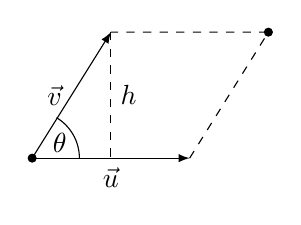
\begin{tikzpicture}[scale=1, transform shape]
		\tikzset{>=latex}
		\coordinate (0) at (0,0);
		\coordinate (P) at (2,0);
		\coordinate (Q) at (1,1.6);
		\coordinate (E) at (3,1.6);
		\draw [->] (0) -- node[midway,below] {$\vec{u}$} (P);
		\draw [->] (0) -- node[midway,left] {$\vec{v}$} (Q);
		\draw [dashed] (P) -- (E) -- (Q);
		\draw [dashed] (Q) -- node[midway,right] {$h$} (1,0);
		% \draw ($(P)!-1cm!(P0)$)  -- (P) node [below]  {$P$} -- (P0) node [above] {$P_0$} -- ($(P0)!-1cm!(P)$) node [left] {$L$};
		% \draw [thick,->,color=blue] (P0) --coordinate [pos={1/2}] (m) node [above] {${\vec{d}}$} ($(P)!1cm!(P0)$);
		% \draw[dashed,->] (0) -- (P);
		% \filldraw (P) circle (0.05);
		% \filldraw (P0) circle (0.05);
		\draw ([shift=(30:0)]0.6,0) arc (0:59:0.6);
		\filldraw (0) circle (0.05);
		\filldraw (E) circle (0.05);
		\node at (0.35,0.2) {$\theta$};
	    \end{tikzpicture}
	\end{center}
	\pause
	Since $\sin\theta =\frac{h}{||\vec{v}||}$, we see that
	$h=||\vec{v}||\sin\theta$.
	\pause
	Therefore, the area is
	\[ ||\vec{u}||~||\vec{v}||\sin\theta.\]
    \myQED\end{proofnoend}

    % \begin{picture}(3,0.6)
    %     \put(1.6,0.1){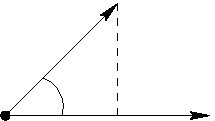
\includegraphics[scale=.6]{figures/vectors-21.pdf}}
    %     \put(1.8,0.4){\scriptsize $\vec{v}$}
    %     \put(1.9,0.0){\scriptsize $\vec{u}$}
    %     \put(1.75,0.15){\scriptsize $\theta$}
    %     \put(2.1,0.3){\scriptsize $h$}
    % \end{picture}
    %
}
%-------------- end slide -------------------------------%}}}
%-------------- start slide -------------------------------%{{{ 9
\frame{
\begin{theorem}
    The volume of the parallelepiped determined by the three
    vectors $\vec{b}$, $\vec{c}$, and $\vec{a}$ in $\RR^3$ is
    \[ |\vec{a}\dotprod(\vec{b}\times\vec{c})|.\]
\end{theorem}
\vfill
\begin{center}
    \includegraphics[scale=0.04]{./figures/Parallelepiped_volume.png}
\end{center}
\vfill
\begin{proof}
		Volume $=$ \textcolor{magenta}{base area} $\times \textcolor{yellow}{h}$,
		where base area $=\textcolor{magenta}{|\vec{b}\times \vec{c}|}$ and
		the height $h= \textcolor{yellow}{|\vec{a}| |\cos(\alpha)|}$. Hence,
		\begin{align*}
				\text{Vol} = \textcolor{magenta}{|\vec{b}\times \vec{c}|}
				\:\textcolor{yellow}{|\vec{a}| |\cos(\alpha)|}
				= |(\vec{b}\times\vec{c})\dotprod\vec{a}|.
		\end{align*}
\end{proof}
}
%-------------- end slide -------------------------------%}}}
%-------------- start slide -------------------------------%{{{ 10
\frame{
\begin{problem}
    Find the area of the triangle having vertices $A(3,-1,2)$, $B(1,1,0)$ and $C(1,2,-1)$.
\end{problem}
\medskip
\pause
\begin{solution}
    The area of the triangle is half the area of the parallelogram defined by $\overrightarrow{AB}$ and $\overrightarrow{AC}$.
    \pause
    $\overrightarrow{AB}= \left[\begin{array}{r} -2 \\ 2 \\ -2 \end{array}\right]$ and
    $\overrightarrow{AC}= \left[\begin{array}{r} -2 \\ 3 \\ -3 \end{array}\right]$.
    \pause
    Therefore
    \[ \overrightarrow{AB}\times\overrightarrow{AC} = \left[\begin{array}{r} 0 \\ -2 \\ -2 \end{array}\right],\]
    \pause
    so the area of the triangle is $\frac{1}{2}||\overrightarrow{AB} \times\overrightarrow{AC}||= \sqrt{2}$.
    \myQED
\end{solution}
}
%-------------- end slide -------------------------------%}}}
%-------------- start slide -------------------------------%{{{ 11
\frame{
\begin{problem}
    Find the volume of the parallelepiped determined by the vectors
    $\vec{u}= \left[\begin{array}{r} 2 \\ 1 \\ 1 \end{array}\right]$,
    $\vec{v}= \left[\begin{array}{r} 1 \\ 0 \\ 2 \end{array}\right]$,
    and
    $\vec{w}= \left[\begin{array}{r} 2 \\ 1 \\ -1 \end{array}\right]$.
\end{problem}
\medskip
\pause
\begin{solution}
    The volume of the parallelepiped is
    \[ |\vec{w}\dotprod(\vec{u}\times\vec{v})| =
	\left|\det\left[ \begin{array}{rrr}
		2 & 1 & 2 \\
		1 & 0 & 1 \\
		1 & 2 & -1
	\end{array}\right]\right|
	=2.
    \]
\end{solution}
}
%-------------- end slide -------------------------------%}}}
\end{document}
